\documentclass[11pt]{article}

\usepackage{url}
\usepackage{hyperref}
\usepackage{graphicx}
\usepackage{verbatim}
\usepackage{color}
\usepackage{upquote}
\usepackage{float}
\usepackage{amsmath}
\usepackage{mwe}
\usepackage{subcaption}
\usepackage{tabulary}

\setlength{\parskip}{0.5cm plus4mm minus3mm}
\captionsetup{font=footnotesize}


\textwidth=6.4in
\textheight=8.5in
\hoffset=-0.7in
\voffset=-0.7in

\setlength{\parindent}{0cm} 

\newcolumntype{L}[1]{>{\raggedright\arraybackslash}p{#1}}
\newcommand{\Yfun}{Y}
%\newcommand{\TAG}{test}
\newcommand{\TAG}{\begin{color}{blue}This tutorial is currently under construction. Please check back later for more by keeping your software updated.\end{color}}

\newcommand{\HERE}{\begin{color}{blue}Currently working on this part.\end{color}}

\hyphenation{Text-Wrangler}

\title{Chapter 4: Vector Spherical Harmonics}
\author{Sarah Kroeker, Alain Plattner, and Kylee Ford}

\begin{document}
\maketitle

\section{Introduction to Vector Spherical Harmonics}

We now will show how the Slepian software can be used to plot vector spherical harmmonics. In Chapters 3 an 4 Classical Vector Slepian Functions and Altitude Cognizant Gradient Vector Slepian Functions will be discussed respectively. 

In Chapter 1 we discussed scalar spherical harmonics, which provide a value for the radial component of a potential field on every point of the defined theta-phi grid. Now we have vector fields which we define as having an intensity and a direction for every point, for example a flow field, magnetic field, or gravity field. There are three basis directions in which the step length is calculated to represent the vector at each point.   

An example of three basis directions on a planets surface could be 1. the radial component (pointing outward from/perpendicular to the planet's surface) 2. the colatitudinal component (Southward) and 3. the longitudinal component (Eastward). 

\begin{figure}[H]
  \centering
  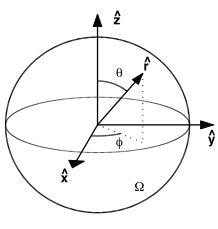
\includegraphics[height=2in]{figures/vectorsphere.png}
  \caption{A sketch of the basis directions on a sphere or planet's surface. $\hat{r}$ is the radial component, $\theta$ is the Southward component, and $\phi$ is the Eastward component, all of which are mutually orthonormal. \textit{Image taken from Figure 1 of Plattner and Simons 2014.}}
\label{figure1}
\end{figure}


\subsection{Different Representations}

There are two particular representations of vector spherical harmonics used in the Slepian software which we will refer to as Type I and Type II and have defined in Table 1 below.

\begin{table}[H]
\caption{Vector Spherical Harmonics Representations}
\begin{tabulary}{\linewidth}{L{7cm}|L{8cm}}
\textbf{Type I} & \textbf{Type II} \\ \hline
   \textbf{Plm} - radial vector spherical harmonics & \textbf{Elm} - vector components that arise from the gradient of a potential field from the planet \\
   \textbf{Blm} - tangential vector spherical harmonics & \textbf{Flm} - vector components that arise from the gradient of a potential field from outside the satellite radius (space) \\
   \textbf{Clm}- divergence free tangential vector spherical harmonics (do not arise from potential fields) & \textbf{Clm} - same as in Type I representation
\end{tabulary}
\end{table}

\section{Type I Representation}

We will mirror the examples in Chapter 1's discussion of scalar spherical harmonics by first plotting a few of the Type I vector spherical harmonics.

Run:

\verb|		demos_chapter_four(4.1)|

\section{Type II Representation}


[kylee's section will be inserted] \\

\TAG
\end{document}
